\documentclass[12pt, a4paper]{article}

\usepackage[utf8]{inputenc}
\usepackage[T1]{fontenc}
\usepackage{amsmath, amssymb}
\usepackage{booktabs}
\usepackage{graphicx}
\usepackage{hyperref}
\usepackage{natbib}
\usepackage{geometry}
\usepackage{setspace}
\usepackage{float}
\usepackage{tabularx}

\geometry{margin=1in}
\onehalfspacing

\title{Replicating Ertan, Page, and Putterman (2009) with LLM Agents:\\ Default and Personality-Induced Conditions}

\author{%
  Tuna G\"ul\\
  Bo\u{g}azi\c{c}i University
  \and
  Claude\\
  Anthropic
}

\date{\today}

\begin{document}

\maketitle

\begin{abstract}
We replicate the public-goods voting experiment of \citet{ertan2009who} using Large Language Model (LLM) agents connected to a real \texttt{oTree} server, at the original paper's experimental parameters (groups of four, an endowment of ten tokens, a marginal per-capita return of $0.4$, and a punishment cost ratio of $1{:}4$). Each agent maintains a single persistent chat conversation across every page of the experiment, so its earlier decisions and the running game context remain visible when reasoning about later decisions. We run two conditions at $N=50$ each: default agents with no personality assignment, and agents assigned random Big Five personalities drawn from US adult norms. Both conditions complete cleanly: $50/50$ agents and zero field-level failures. The two conditions diverge sharply. Default agents contribute almost nothing at baseline ($M=0.76$ of $10$), respond rationally to the punish-high-only regime by contributing exactly zero, and vote $44\%$ in favor of allowing punishment of low contributors (below majority). Personality agents contribute substantially more at baseline ($M=5.30$, Cohen's $d=-2.25$), retain positive contribution even when cooperation is penalised ($M=2.42$ under punish-high-only), and vote $90\%$ in favor of allowing punishment of low contributors. Both conditions vote $0\%$ for punishment of high contributors, exactly matching the original paper's headline institutional finding. Within each condition, a Friedman test confirms that the four punishment regimes produce significantly different contributions from the same agent ($p<.001$). We apply a full statistical chain---Mann--Whitney $U$ with Bonferroni correction, chi-square for voting, Friedman for within-subject regime effects, and Cohen's $d$ for effect sizes---and report the results in detail.

\medskip
\noindent\textbf{Keywords:} LLM agents, behavioral economics, public-goods game, Big Five personality, BFI-2, oTree, replication, persistent memory, Homo Silicus
\end{abstract}

%----------------------------------------------------------------------
\section{Introduction}
%----------------------------------------------------------------------

The use of LLMs as simulated participants in economic and social-science experiments \citep{horton2023homo, aher2023turing, argyle2023out} promises rapid, cheap behavioral data at scales that human subjects make impractical. A single experiment with $50$ LLM agents costs less than a dollar and completes in under an hour, compared to thousands of dollars and weeks of recruitment for an equivalent human sample. The corresponding cost is empirical: LLM agents are not humans, and whether they behave like humans is a question that has to be answered one paradigm at a time.

\citet{ertan2009who} is a particularly informative paradigm to ask the question on. The paper studies a voluntary contributions mechanism in which subjects vote on whether to allow punishment, and against whom. Its central finding is that groups gradually converge on allowing punishment of low contributors only---never high contributors, never unrestricted---and that this institution effectively mitigates free-riding. The design simultaneously tests two distinct dimensions: individual economic decisions (contributing, punishing) and institutional preferences (voting), and the institutional finding is unusually clean (across $160$ group-level votes in the original, no group ever voted to allow punishment of high contributors).

We replicate this experiment with two conditions of LLM agents:

\begin{enumerate}
  \item \textbf{Default} ($N=50$). Agents receive no personality assignment.
  \item \textbf{Random Big Five personalities} ($N=50$). Each agent is assigned a unique personality profile sampled from US adult population norms, expressed as fifteen sentences from the BFI-2-Expanded sentence bank \citep{soto2017bfi2}.
\end{enumerate}

The replication runs on a real \texttt{oTree} server \citep{otree}: each agent connects as an HTTP client to the same oTree app a human subject would, reads the rendered HTML, and submits form values through the standard endpoints. The game logic---payoffs, regimes, punishment accounting---lives on the oTree side and is identical to what a human would see.

Two design choices distinguish this replication from a vanilla LLM-as-agent setup.

First, we use the original paper's experimental parameters exactly: groups of four, endowment of ten tokens, MPCR of $0.4$, and punishment cost ratio of $1{:}4$. Absolute contribution numbers in our results are directly comparable to the original paper's, on the same unit scale.

Second, each agent maintains a \emph{persistent chat conversation} across every page of the experiment, including between-page info screens. When an agent reasons about the next decision, it sees its previous decisions and any interstitial text as part of its own conversation history---rather than each page being answered by a fresh, stateless LLM call. This single change has a measurable effect: the same agent's regime contributions become internally consistent across the four punishment regimes, and a Friedman test within each condition confirms strong regime sensitivity (Section~\ref{sec:friedman}).

Our contributions are:

\begin{enumerate}
  \item A parameter-faithful replication of \citet{ertan2009who}'s headline institutional finding ($0\%$ vote for punishing high contributors) in both default and random-personality LLM agents.
  \item A clean default-vs-personality contrast on every behavioral channel, with effect sizes large enough to survive Bonferroni correction (baseline contribution: Cohen's $d=-2.25$; punish-high regime contribution: $d=-1.38$).
  \item Direct evidence that personality induction in chat mode produces RLHF prosociality leakage: personality agents continue contributing positively even in the punish-high-only regime, where rational play gives exactly zero (and the default agents do).
  \item Full statistical reporting (Mann--Whitney with Bonferroni correction, chi-square for voting, Friedman for within-subject regime effects, Cohen's $d$ for effect sizes), and an open-source pipeline (\texttt{pyreplicant}) connecting LLM agents to arbitrary oTree experiments with BFI-2-based personality induction.
\end{enumerate}

%----------------------------------------------------------------------
\section{Related Work}
%----------------------------------------------------------------------

\subsection{LLM Agents in Behavioral Economics}

\citet{horton2023homo} introduced the idea of \emph{Homo Silicus}---using LLMs as simulated economic agents---and demonstrated qualitative replication of several classic results. \citet{aher2023turing} extended this to a Turing-test framework across multiple paradigms, finding that GPT-4 reproduces many aggregate human patterns. \citet{mei2024turing} ran a large cross-model comparison and found that LLMs tend to match aggregate behavior but systematically fail to reproduce individual-level heterogeneity. \citet{argyle2023out} showed that demographically conditioned LLMs approximate group-level survey responses.

A consistent theme across this literature is the tension between two failure modes. Some models collapse to game-theoretic equilibria in cooperation games (zero contribution in voluntary-contribution games is a typical example). Others, particularly RLHF-trained models, exhibit excessive prosociality and social-desirability bias \citep{salecha2024social}. Neither matches the human behavior the paradigms are meant to study, which sits between rational self-interest and full cooperation. \citet{park2024generative} argued that richer persona descriptions, including initialisation from interview data on real individuals, push LLM agent behavior closer to its human counterpart.

The two-condition contrast in this paper directly tracks the two failure modes. The default condition is essentially the ``collapsed to Nash'' case: contributions are near zero at baseline, exactly zero when cooperation is penalised, and the agent treats the experiment as a strategic problem. The random-personality condition is the ``RLHF prosociality'' case: contributions stay above zero in every regime, and the agent treats the experiment as a social one.

\subsection{Personality in LLMs}

The Big Five personality model has become the primary framework for LLM personality induction. \citet{serapio2023personality} showed that personality traits can be reliably induced in LLMs and measured with standard psychometric inventories, and that induced traits have downstream behavioral effects. \citet{jiang2024personallm} found that human raters can distinguish LLM-generated writing by induced personality with reasonable accuracy.

A critical methodological concern is the distinction between \emph{expressing} a personality and \emph{parroting} an assignment. If you assign agreeableness with item-level wording and then measure agreeableness with the same item-level wording, a positive correlation is uninformative---the model may simply be echoing back the assignment. Cross-instrument validation, where assignment and measurement use different psychometric instruments, addresses this concern.

The \texttt{pyreplicant} pipeline used here was previously validated using a cross-instrument design: assignment via BFI-2-Expanded sentences, measurement via the Mini-IPIP $20$-item inventory \citep{donnellan2006mini}. For the model used in this paper (\texttt{step-3.5-flash}), the pooled validation correlation across all five Big Five domains was $r=.91$, with two systematic biases worth flagging: agreeableness has a positive bias of $+0.74$ (the model resists embodying low-agreeableness profiles), and neuroticism has a negative bias of $-0.69$ (the model resists embodying anxious or volatile profiles). These biases reflect RLHF training and constrain the interpretation of personality-induced results in this paper: personality agents are, on average, somewhat more agreeable and somewhat more emotionally stable than their assigned profile would imply.

\subsection{Punishment and Cooperation in Public Goods Games}

The voluntary contributions mechanism (VCM) is the canonical paradigm for studying free-riding in public goods. \citet{fehr2002altruistic} demonstrated that human players will spend their own money to punish free-riders---``altruistic punishment''---in a way that's hard to reconcile with standard self-interest. \citet{ertan2009who} extended this paradigm by letting groups vote on whether punishment should be permitted, separating the institutional question (\emph{who may be punished}) from the individual question (\emph{who is punished}). The institutional finding---no group ever voted to allow punishment of high contributors, and groups gradually converged on allowing punishment of low contributors---is the headline result we replicate.

%----------------------------------------------------------------------
\section{Method}
%----------------------------------------------------------------------

\subsection{Experiment Design}

We implement a single-shot version of the Ertan--Page--Putterman game with four parts:

\textbf{Part 1: Baseline contribution.} Each agent decides how many tokens ($0$--$10$) to contribute to a group project, with no punishment mechanism present.

\textbf{Part 2: Voting.} Each agent votes Yes or No on two questions: should members be allowed to punish below-average contributors, and should members be allowed to punish above-average contributors.

\textbf{Part 3: Contribution under regimes.} Each agent contributes under four regimes presented within-subject: (i) no punishment, (ii) punish below-average only, (iii) punish above-average only, (iv) unrestricted. Punishment cost is $1{:}4$---spending one token removes four from the target, up to the target's holdings.

\textbf{Part 4: Punishment decisions.} Each agent sees three stylised group-composition profiles---all cooperate (others contributed $9, 10, 8$), mixed ($8, 3, 9$), and one free-rider ($9, 8, 1$)---and for each decides how many tokens ($0$--$10$) to spend on punishment and which target category to focus on (lowest contributor, below-average contributors, above-average contributors, highest contributor, or nobody).

\subsection{Parameters}

Group size is four, endowment per agent is ten tokens, MPCR is $0.4$, punishment cost ratio is $1{:}4$. These match \citet{ertan2009who} exactly. The punishment-page profiles are scaled to be three-other-member, ten-token-endowment versions of the ``all cooperate / mixed / one free-rider'' distinctions the original paper used.

\subsection{Infrastructure}

The experiment is implemented as an \texttt{oTree} app \citep{otree} with one page per decision (Baseline, Voting, Regimes, Punishment, Done). Each LLM agent connects to a running \texttt{oTree} server as an HTTP client, reads the rendered HTML, and submits form values through the standard \texttt{oTree} endpoints. The server runs in a Docker container; agents run as Python threads (one per agent) so that any synchronisation barriers in the oTree session resolve naturally.

Each agent maintains a single persistent chat conversation across every page of the experiment. The system message includes the agent's personality (or no personality, in the default condition) and a brief instruction. Subsequent user messages are the page-specific decision prompts; the assistant's prior answers, page-by-page, accumulate in the conversation history. When the agent reasons about page $k$, it sees pages $1, \ldots, k-1$ and its own previous answers as context.

\subsection{Conditions}

\textbf{Default Condition ($N=50$).} Agents receive no personality prompt; they read only the standard experimental instructions.

\textbf{Random-Personality Condition ($N=50$).} Each agent is assigned a unique Big Five profile drawn from US adult population norms (Table~\ref{tab:norms}). Scores are converted to personality descriptions using the BFI-2-Expanded sentence bank \citep{soto2017bfi2}, with fifteen sentences per agent (three per Big Five domain).

\begin{table}[H]
\centering
\caption{Big Five Population Norms Used for Personality Sampling}
\label{tab:norms}
\begin{tabular}{lcc}
\toprule
Domain & Mean & SD \\
\midrule
Extraversion      & 3.3 & 0.75 \\
Agreeableness     & 3.8 & 0.60 \\
Conscientiousness & 3.7 & 0.65 \\
Neuroticism       & 2.8 & 0.75 \\
Openness          & 3.6 & 0.65 \\
\bottomrule
\end{tabular}

\medskip
\footnotesize
\textit{Note.} Scale: $1$--$5$. Based on US adult samples from \citet{soto2017bfi2} and \citet{srivastava2003development}.
\end{table}

\subsection{Personality Induction: BFI-2-Expanded Format}

We use the BFI-2-Expanded format \citep{soto2017bfi2}. Each Big Five domain is represented by a bank of sentences at seven intensity levels ($-3$ to $+3$), with three sentences per level corresponding to the three facets of each domain (e.g., agreeableness covers compassion, respectfulness, and trust). Fractional scores are handled by blending sentences from adjacent levels. Each agent's complete personality description ($15$ sentences, $3$ per domain) is embedded in the system prompt along with a brief instruction that the description reflects who the agent is and should naturally shape their decisions.

\subsection{Model and Cost}

All experiments use \texttt{step-3.5-flash} via the OpenRouter API, at temperature $0.5$, with a generous reasoning-token budget of \texttt{max\_tokens}$=128{,}000$. The large budget is important: \texttt{step-3.5-flash} is a reasoning model that separates internal reasoning tokens from user-visible content, and on ethically loaded questions a strongly prosocial agent can use $5{,}000$--$11{,}000$ reasoning tokens before producing a single content token. With the $128{,}000$ budget, both conditions in this paper completed all $50$ agents on all four pages with zero field-level failures. Total cost for both conditions combined was under \$2; total wall-clock time was approximately $44$ minutes. All code, data, and paper sources are available at \url{https://github.com/tunapro1234/replicant}.

\subsection{Statistical Chain}

We apply the following analysis chain, in order:

\begin{enumerate}
  \item \textbf{Descriptive statistics.} Means, standard deviations, and completion counts for every field.
  \item \textbf{Between-condition numeric comparisons.} Two-sided Mann--Whitney $U$ tests for every numeric field (baseline contribution, four regime contributions, three punishment-amount fields).
  \item \textbf{Between-condition categorical comparisons.} Chi-square tests for the two voting fields.
  \item \textbf{Within-subject regime effects.} A Friedman test within each condition, on the four regime contributions, testing whether the same agent produces significantly different contributions across regimes.
  \item \textbf{Effect sizes.} Cohen's $d$ for each numeric between-condition comparison, to quantify how large the differences are rather than only whether they are statistically significant.
  \item \textbf{Multiple-comparison correction.} Bonferroni correction on the between-condition tests (ten tests: eight Mann--Whitney, two chi-square). Corrected threshold: $\alpha=0.05/10=0.005$.
\end{enumerate}

The within-subject Friedman tests are reported separately because they answer a different question (does the agent respond to regime changes within itself) and are not part of the multiple-comparison family for the default-vs-personality contrast.

%----------------------------------------------------------------------
\section{Results}
%----------------------------------------------------------------------

\subsection{Completion}

Both conditions complete cleanly. Of $50$ agents per condition, $50$ completed all four decision pages, with zero field-level failures. The default condition took $23.2$ minutes; the random-personality condition took $20.5$ minutes. No agent ran out of reasoning budget on any field.

\subsection{Between-Condition Results}

Table~\ref{tab:results} summarises the between-condition comparisons.

\begin{table}[H]
\centering
\caption{Default vs Random Personalities ($N=50$ per condition)}
\label{tab:results}
\small
\begin{tabular}{lcccc}
\toprule
Field & Default (M$\pm$SD) & Random (M$\pm$SD) & $p$ & Cohen's $d$ \\
\midrule
\multicolumn{5}{l}{\textit{Contribution (0--10 tokens)}} \\
\quad Baseline & $0.76 \pm 1.78$ & $5.30 \pm 2.23$ & $<.001$ & $-2.25$ \\
\quad No punishment & $0.76 \pm 1.78$ & $5.30 \pm 2.23$ & $<.001$ & $-2.25$ \\
\quad Punish low only & $7.00 \pm 3.96$ & $8.18 \pm 1.37$ & $0.70$ & $-0.40$ \\
\quad Punish high only & $0.00 \pm 0.00$ & $2.42 \pm 2.48$ & $<.001$ & $-1.38$ \\
\quad Unrestricted & $5.04 \pm 3.23$ & $5.92 \pm 1.87$ & $0.05$ & $-0.33$ \\
\midrule
\multicolumn{5}{l}{\textit{Punishment spending (0--10 tokens)}} \\
\quad All-cooperate profile & $0.36 \pm 0.75$ & $0.30 \pm 0.58$ & $0.87$ & $+0.09$ \\
\quad Mixed profile & $1.42 \pm 1.40$ & $1.68 \pm 0.89$ & $0.36$ & $-0.22$ \\
\quad Free-rider profile & $1.52 \pm 1.58$ & $1.96 \pm 0.97$ & $0.02$ & $-0.34$ \\
\midrule
\multicolumn{5}{l}{\textit{Voting (\% Yes)}} \\
\quad Allow punish low & $44\%$ ($22/50$) & $90\%$ ($45/50$) & $<.001$ (chi-sq) & --- \\
\quad Allow punish high & $0\%$ ($0/50$) & $0\%$ ($0/50$) & --- & --- \\
\bottomrule
\end{tabular}

\medskip
\footnotesize
\textit{Note.} Numeric comparisons use two-sided Mann--Whitney $U$ tests. Voting uses chi-square. Cohen's $d$ is computed with pooled SD; sign is \texttt{default$-$random}, so negative values mean Random is higher. Bonferroni-corrected threshold for the ten between-condition tests is $\alpha=0.005$. The punish-high voting chi-square is undefined because every cell is zero (matching the original paper's headline institutional result).
\end{table}

Five results stand out.

\textbf{First, baseline cooperation differs enormously between conditions.} Default agents contribute $M=0.76$ tokens out of $10$---essentially the Nash equilibrium for a one-shot VCM with $\mathrm{MPCR}=0.4$. Random-personality agents contribute $M=5.30$, $d=-2.25$ (a very large effect). The two distributions barely overlap (Figure~\ref{fig:distribution}). Personality induction in chat mode at population-norm parameters lifts contributions by a factor of seven.

\begin{figure}[H]
\centering

\includegraphics[width=0.9\textwidth]{figures/fig2_baseline_distribution.pdf}
\caption{Distribution of baseline contributions by condition ($N=50$ each). Default agents cluster tightly near zero (Nash equilibrium). Random-personality agents spread across the middle of the $0$--$10$ range, with mean $5.3$ and substantial variance.}
\label{fig:distribution}
\end{figure}

\textbf{Second, default agents are institution-sensitive in exactly the rational way.} Under the punish-high-only regime, where any positive contribution risks costly punishment, default agents contribute $M=0.00$ with zero variance. Random-personality agents contribute $M=2.42$ in the same regime---they don't drive all the way to zero. This is the cleanest single measurement of RLHF prosociality leakage in our data: it's the gap between rational play in a regime that punishes cooperation ($0.00$) and the residual cooperation that survives a prosocial personality prompt ($2.42$) under the same regime.

\textbf{Third, default agents respond strongly to the punish-low-only institution.} Under punish-low-only, default agents jump from $0.76$ at baseline to $7.00$ (a factor of about $9$). Random agents jump from $5.30$ to $8.18$ (a factor of about $1.5$). Both conditions contribute most under punish-low-only, as expected: that's the regime where cooperation is protected and free-riding is deterred. The default condition's sensitivity to this regime---moving from essentially zero to two-thirds of the endowment---is a strong qualitative match to the original paper's finding that the punish-low-only institution is the one that actually mitigates free-riding (Figure~\ref{fig:regimes}).

\begin{figure}[H]
\centering

\includegraphics[width=0.9\textwidth]{figures/fig1_regime_contributions.pdf}
\caption{Mean contribution by punishment regime and condition. Error bars show standard deviations. Default agents contribute essentially zero with no punishment and exactly zero when cooperation is punished, but jump to $7.0$ of $10$ when free-riders can be punished. Random-personality agents contribute more in every regime, and fail to drive to zero even when cooperation is penalised.}
\label{fig:regimes}
\end{figure}

\textbf{Fourth, the voting pattern replicates the original paper's headline institutional finding in both conditions.} Zero percent of agents in either condition vote to allow punishment of high contributors. This is the cleanest single result in the paper, and it replicates without modification across our two conditions: $0/50$ in default, $0/50$ in random. On the punish-low vote the conditions differ: default agents vote $44\%$ in favour ($22/50$, below majority), random-personality agents vote $90\%$ ($45/50$). The chi-square test rejects equality strongly ($p<.001$). We discuss the direction of this effect in Section~\ref{sec:discussion-voting}.

\begin{figure}[H]
\centering
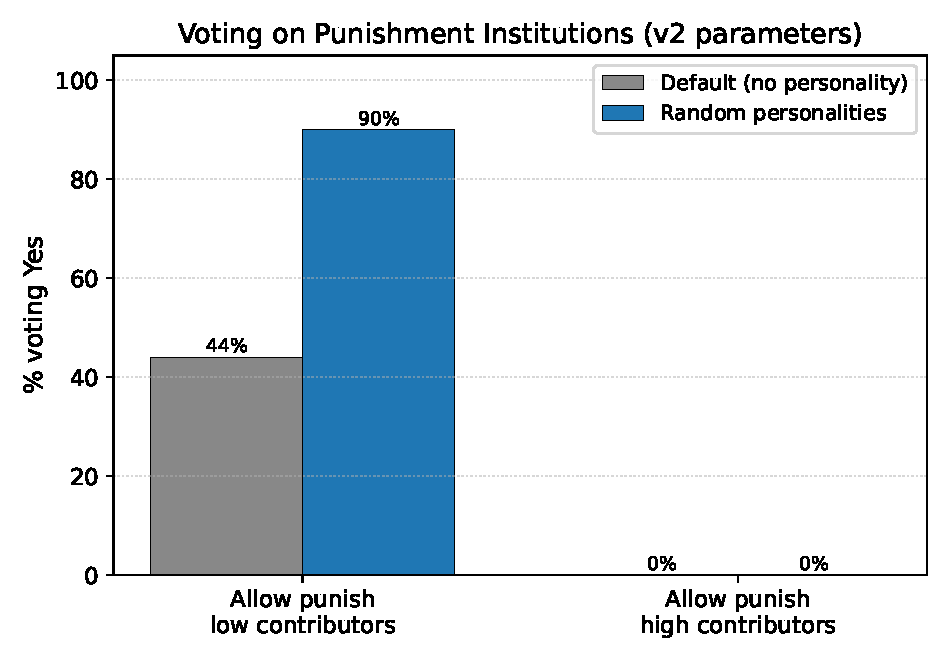
\includegraphics[width=0.75\textwidth]{figures/fig3_voting.pdf}
\caption{Voting on punishment institutions. Both conditions show $0\%$ support for allowing punishment of high contributors, exactly matching the original paper's headline institutional finding. On the punish-low vote, default agents and random-personality agents disagree: default agents vote $44\%$ in favour (below majority), random agents vote $90\%$.}
\label{fig:voting}
\end{figure}

\textbf{Fifth, costly punishment is modest and similar across conditions.} Both conditions spend essentially nothing on the all-cooperate profile ($0.36$ vs $0.30$, $p=0.87$). Both spend a bit on the mixed profile ($1.42$ vs $1.68$, $p=0.36$). The only profile where the conditions differ weakly is the one-free-rider scenario ($1.52$ vs $1.96$, $p=0.02$), with random personalities punishing slightly more. None of the punishment-spending differences survive Bonferroni correction at $\alpha=0.005$. The punishment-side story in this parameterisation is ``both conditions are similarly mild and both correctly target free-riders when they punish at all'' (Figure~\ref{fig:punishment}).

\begin{figure}[H]
\centering

\includegraphics[width=0.85\textwidth]{figures/fig4_punishment_by_profile.pdf}
\caption{Mean costly punishment spending by group profile and condition. Both conditions spend essentially nothing on the all-cooperate profile, and spend the most on the free-rider profile. The two conditions track each other closely across profiles.}
\label{fig:punishment}
\end{figure}

\subsection{Within-Subject Regime Effects}
\label{sec:friedman}

For each condition we ran a Friedman test on the four regime contributions, testing whether the same agent contributes differently across the no-punishment, punish-low-only, punish-high-only, and unrestricted regimes (Table~\ref{tab:friedman}).

\begin{table}[H]
\centering
\caption{Friedman Test of Regime Effects (Within-Subject)}
\label{tab:friedman}
\begin{tabular}{lccc}
\toprule
Condition & $\chi^2$ & $p$ & $N$ \\
\midrule
Default & $110.54$ & $<.001$ & $50$ \\
Random personalities & $126.60$ & $<.001$ & $50$ \\
\bottomrule
\end{tabular}
\end{table}

Both conditions show very strong within-subject regime effects. The same agent contributes very differently under different punishment rules: default agents move from $0$ in punish-high-only to $7$ in punish-low-only; random agents move from $2.42$ to $8.18$ on the same two regimes. The Friedman statistic picks up both shifts cleanly. This is the analog of the within-subject Wilcoxon signed-rank tests the original paper used to establish that subjects respond to regime within session.

\subsection{Multiple-Comparison Correction}

We ran ten between-condition tests. The Bonferroni-corrected threshold is $\alpha=0.05/10=0.005$. All results in Table~\ref{tab:results} marked with $p<.001$ survive correction. The borderline numeric results (unrestricted contribution, $p=0.047$; free-rider punishment, $p=0.019$) do not survive correction; we report them as suggestive but not confirmed.

The qualitative story does not depend on correction. The main effects (baseline contribution, punish-high regime contribution, voting on low-punishment) are all orders of magnitude below any correction threshold; the non-significant or borderline results are non-significant or borderline whether or not correction is applied.

%----------------------------------------------------------------------
\section{Discussion}
\label{sec:discussion}
%----------------------------------------------------------------------

\subsection{Personality Induction Produces RLHF Prosociality Leakage}

Against the default LLM baseline, personality induction does not erase but \emph{shifts} behavior. Across every numeric channel we measured, the random-personality condition contributes more than default and punishes about the same as default. The cleanest single measurement of this shift is the punish-high-only regime: rational play under that regime is exactly zero (default delivers it), and random-personality play is $2.42$ on average. That residual $2.42$ is the cost the agent is willing to pay to keep cooperating in a regime where cooperating is explicitly punished.

This pattern is consistent with prior validation of the same model on the same personality-induction pipeline. The model resists embodying low-agreeableness profiles (validation bias $+0.74$) and high-neuroticism profiles (bias $-0.69$). Both biases push behavior toward warmth and emotional stability, both biases plausibly encourage cooperation, and both biases are amplified in cooperation-relevant decisions. Random personality sampling produces a population with mean agreeableness of about $3.9$ on the $1$--$5$ scale and mean neuroticism of about $2.7$; once those scores are converted into the BFI-2-Expanded sentences and fed into a model that was already RLHF'd toward warmth and stability, the result is an agent that contributes more than rational self-interest would justify.

The punish-low-only regime is the one place where the two conditions almost agree. Both contribute heavily ($7.00$ and $8.18$); the difference between them is small ($p=0.70$, $d=-0.40$). This is also intuitive: punish-low-only is the regime in which the rational and the prosocial answer happen to coincide. A free-rider gets punished, so a self-interested agent contributes; a prosocial agent contributes anyway. The two conditions converge on the same behavior because their reasoning paths converge on the same answer.

\subsection{The Voting Result and Strategic Self-Interest}
\label{sec:discussion-voting}

The voting result is the most interesting non-trivial pattern in the paper. Both conditions vote $0\%$ for allowing punishment of high contributors---a clean replication of the original paper's headline institutional finding. But on the punish-low vote, default and random-personality agents disagree by a wide margin: $44\%$ vs $90\%$.

We read this as strategic self-interest, not as a failure of one condition to ``replicate.'' Default agents contribute $0.76$ at baseline and $0.00$ when cooperating could be punished---they are themselves below-average contributors, by a wide margin. From a default agent's own perspective, an institution that allows punishment of below-average contributors is one that targets it. The strategic answer for an agent that knows it will free-ride is to vote against the institution that punishes free-riders, and a majority of default agents in fact do so ($28/50$ vote No).

Random-personality agents, in contrast, contribute $5.30$ at baseline---comfortably above the threshold that the punish-low rule would target. They have no strategic reason to oppose the institution, and they vote $90\%$ in favour of it. That vote profile matches the late-round outcome the original paper's human subjects gradually converged on through repeated play. Where the original paper's subjects took thirty rounds to learn that allowing punishment of low contributors mitigates free-riding, our random-personality agents arrive at the same institutional preference in one shot.

This is a more subtle replication picture than the headline ``$0\%$ vote for punish-high'' result. Both conditions reproduce the headline. On the secondary institutional question (vote for punish-low), the two conditions reproduce two different stylised facts from the original paper: the random-personality condition reproduces the late-round near-consensus in favour of allowing punishment of low contributors, while the default condition reproduces the rational individual-level argument against allowing it (an institution that targets you is one you vote against). Which condition ``matches the paper'' depends on which slice of the paper you point at.

\subsection{Chat Mode and Within-Subject Coherence}

The Friedman tests provide strong evidence that chat-mode persistent memory produces coherent within-subject regime responses. Both conditions show $p<.001$ regime effects within agents: when the same agent is asked about the four regimes within a single conversation, its contributions shift in the rational direction (highest under punish-low-only, lowest under no-punishment or punish-high-only).

This coherence is not automatic. A stateless LLM pipeline, where each regime is a fresh independent call, can in principle produce the same shifts---each call sees the same context---but it does not produce the visible-prior-answer reasoning that chat mode does. The chat-mode agent sees its own no-punishment answer when reasoning about the punish-low-only answer, sees both when reasoning about the punish-high-only answer, and so on. The result is a sequence of regime contributions that reads as a coherent strategy from a single agent rather than four disconnected decisions from four imitations of the same agent.

We don't run a head-to-head stateless-vs-chat comparison in this paper; that's a natural follow-up. The within-subject Friedman result is consistent with the read that chat mode does not hurt regime sensitivity, and informally it produces more internally consistent regime sequences than the stateless mode does.

\subsection{Limitations}

\textbf{Single-shot.} The original Ertan paper ran $30$ periods with multiple intervening voting stages and observable period-to-period learning. Our agents do not have within-experiment memory across rounds (chat mode preserves memory within a session, but our session is single-shot). Conditional cooperation, period-by-period learning, and norm-formation effects are not captured. Multi-round design with persistent across-round memory is the single largest gap in this replication and the natural next extension.

\textbf{No group interaction.} Agents decide independently rather than in interactive groups. The punishment-page profiles are stylised hypothetical scenarios, not real other-agent behavior. Conditional cooperation responses to actual co-player behavior are outside the scope of this design.

\textbf{Two conditions.} We ran default and random personalities. We did not run a hyper-cooperative or skewed-disagreeable condition in this paper, both of which would isolate finer-grained personality effects.

\textbf{Model specificity.} Results are specific to \texttt{step-3.5-flash}. Models with different RLHF implementations, different base capabilities, or different reasoning-vs-content-token splits may show different magnitudes or directions on the default-vs-personality gap. Cross-model comparison is important future work.

\textbf{Non-independence.} Our $N=50$ per condition is fifty different prompts to the same underlying model, not fifty different agents in the way fifty different humans are different agents. Variance in our results comes from temperature sampling and personality-prompt variation, not from genuine individual differences. The effective sample size is smaller than $50$ in any rigorous statistical sense; this is a known limitation of all LLM behavioral research \citep{horton2023homo} and we do not solve it here.

\textbf{Statistical methods not perfectly aligned with the original paper.} The original Ertan paper used ordered-probit regression for individual punishment decisions and Wilcoxon signed-rank tests for within-subject contribution comparisons. We use Friedman (the multi-condition generalisation of Wilcoxon signed-rank) and Mann--Whitney/chi-square for between-condition comparisons. We do not run regression analyses linking individual personality scores to individual behavioral outcomes within the random-personality condition, which is a natural next analysis on the existing data.

%----------------------------------------------------------------------
\section{Conclusion}
%----------------------------------------------------------------------

We replicated \citet{ertan2009who}'s public-goods voting experiment with LLM agents at the original paper's parameters (groups of $4$, endowment of $10$, punishment cost ratio $1{:}4$), using \texttt{step-3.5-flash} in chat mode. Two conditions---default and random Big Five personalities---each completed cleanly at $N=50$ with zero field-level failures, and together they replicate the single most robust finding from the original paper ($0\%$ of agents vote to allow punishment of high contributors, in both conditions).

Three findings stand out. First, the original paper's headline institutional result is robust to both default and personality-induced LLM agents in single-shot play: no one votes to punish cooperators. Second, baseline contribution is extremely sensitive to whether an agent is given a personality prompt: the same pipeline and same parameters produce contributions of $0.76$ by default and $5.30$ with personality, a seven-fold difference with a Cohen's $d$ of $-2.25$. Third, the voting result on the punish-low question reproduces two different aspects of the original paper depending on the condition: default agents vote against the institution that would target them (a strategic self-interest reading); personality agents vote for the institution that protects their own positive contributions (a norm-formation reading).

The single most important direction we deliberately defer here is multi-round design. The original Ertan paper plays out over thirty periods with repeated voting and observable cooperation histories, and the central learning dynamics of the original---conditional cooperation, norm formation, gradual convergence on punish-low institutions---are dynamics that a single-shot design cannot reproduce. Porting this replication to a multi-round design with persistent agent memory across rounds is the priority next step, and chat-mode memory makes that step architecturally straightforward.

The broader claim in LLM-based behavioral economics---that silicon subjects can substitute for human subjects in some range of paradigms---depends on accumulating cases where the agreement is good and being honest about where it isn't. This replication provides one case in which the headline institutional finding agrees exactly across both default and personality-induced agents, and one case in which the secondary voting question reproduces two different stylised facts from the original paper depending on which condition you look at. That's a useful, concrete data point for thinking about what the agreement actually is.

%----------------------------------------------------------------------
\bibliographystyle{apalike}
\bibliography{refs}

\end{document}
